\chapter{Continuous Random Variables}


% \section{Continuous Sample Space}
\begin{axiom}
    A random variable $X$ is continuous if the sample space $S_X$ consists of one or more intervals. For $x\in S_X$, $P_X(x)=0$.
\end{axiom}


\section{Cumulative Distribution Function (CDF)}
\begin{definition}
    The CDF of continuous random variable $X$ is
    \[F_X(x) = \P{X\leq x}.\]
\end{definition}

\begin{theorem}
    For any random variable $X$,
    \begin{enumerate}
        \item $F_X(-\infty)=0$
        \item $F_X(\infty)=1$
        \item $\P{x_1<X\leq x_2} = F_X(x_2)-F_X(x_1)$
    \end{enumerate}
\end{theorem}


\section{Probability Density Function (PDF)}
Start with a continuous random variable $X$ with CDF $F_X(x)$. The probability of ``$X$ with volume $\triangle$'' is defined as:
\begin{align*}
    \P{x<X\leq x+\triangle}
    &= F_X(x+\triangle)-F_X(x) \\
    &= \frac{F_X(x+\triangle)-F_X(x)}{(x+\triangle)-x}\cdot\triangle.
\end{align*}
\begin{definition}[Probability Density Function (PDF)]
    \begin{align*}
        f_X(x)
        = \lim_{\triangle\rightarrow 0}\frac{F_X(x+\triangle)-F_X(x)}{\triangle}
        = \frac{\diff F_X(x)}{\diff x}.
    \end{align*}
\end{definition}

\begin{theorem}
    For a continuous random variable $X$ with \textnormal{PDF} $f_X(x)$,
    \begin{enumerate}
        \item $f_X(x)\geq 0$ for all $x$
        \item $F_X(u)=\int_{-\infty}^u f_X(x)\diff x$
        \item $\int_{-\infty}^{\infty} f_X(x)\diff x = 1$
    \end{enumerate}
\end{theorem}

\begin{theorem}
    \begin{align*}
        \P{x_1<X\leq x_2}=\int_{x_1}^{x_2}f_X(x)\diff x.
    \end{align*}
\end{theorem}


\section{Expected Value}
\begin{definition}[Expected value]
    \begin{align*}
        \E{X}=\int_{-\infty}^{\infty} xf_X(x) \diff x.
    \end{align*}
\end{definition}

\begin{theorem}
    [Integral Identity]
    For every non-negative random variable $X$, \[\E{X}=\int_{0}^{\infty}1-F_X(u)\diff u=\int_{0}^{\infty}\P{X>u}\diff u.\]
\end{theorem}

\begin{proof}
    \begin{align*}
        \E{X}
        &= \int_{0}^{\infty}xf_X(x)\diff x && \text{($X$ is non-negative)} \\
        &= \int_{0}^{\infty}\parens*{\int_{0}^{x} 1 \diff u} f_X(x)\diff x \\
        &= \int_{0}^{\infty}\parens*{\int_{u}^{\infty}f_X(x)\diff x}\diff u && \text{(Some Algebra)}\\
        &= \int_{0}^{\infty}1-F_X(u)\diff u = \int_{0}^{\infty}\P{X>u}\diff u. && \text{(Definition of CDF)}
    \end{align*}
\end{proof}

\begin{theorem}[Derived Random Variable]
    \begin{align*}
        \E{g(X)} = \int_{-\infty}^{\infty} g(x)f_X(x)\diff x.
    \end{align*}
\end{theorem}

\begin{theorem}
    For any random variable $X$,
    \begin{enumerate}
        \item $\E{aX+b}=a\E{X}+b$,
        \item $\E{X-\mu_x}=0$,
        \item $\Var[X] = \E{X^2}-\mu_x^2$,
        \item $\Var[aX+b]=a^2\Var[X]$.
    \end{enumerate}
\end{theorem}

\section{Families of Continuous Random Variables}
\begin{enumerate}
    \item Continuous Uniform($k$, $l$): A continuous counterpart of Discrete Uniform($k$, $l$){
        \begin{align*}
            f_X(x)
            &= {
                \begin{cases}
                \frac{1}{l-k} & k\leq x \leq l \\
                0             & otherwise.
                \end{cases} } \\
            F_X(x)
            &= \frac{x-k}{l-k}. \qquad x\in (k,l)\\
            \E{X}
            &= (l+k)/2. \\
            \Var[X]
            &= (l-k)^2/12. \\
        \end{align*}
    }
    \item Exponential($\lambda$): Get the $\bm{1}$\textbf{st} success at the $\bm{x}$\textbf{th} unit of time. This is a continuous counterpart of Geometry($p$) where $p=\lim\limits_{\triangle t\rightarrow 0}\lambda\triangle t$ (\ie $\lambda$ is the probability density of success per unit of time) {
        \begin{align*}
            f_X(x)
            &= {
                \begin{cases}
                    \lambda e^{-\lambda x} & x\geq 0 \\
                    0                      & otherwise.
                \end{cases}
            } \\
            F_X(x)
            &= 1-e^{-\lambda x}. \\
            \E{X}
            &= 1/\lambda. \\
            \Var[X]
            &= 1/\lambda^2.
        \end{align*}
    }
    \item Erlang($k$, $\lambda$): Get the $\bm{k}$\textbf{th} success at the $\bm{x}$\textbf{th} unit of time. This is a continuous counterpart of  Pascal($k$,$p$){
        \begin{align*}
            f_X(x)
            &= {
                \begin{cases}
                    \frac{\lambda^kx^{k-1}e^{-\lambda x}}{(k-1)!} & x\geq 0 \\
                    0      & otherwise.
                \end{cases}
            } \\
            F_X(x)
            &= \frac{\gamma(k, \lambda x)}{(k-1)!}. \\
            \E{X}
            &= k/\lambda. \\
            \Var[X]
            &= k/\lambda^2.
        \end{align*}
    }
    \item Gamma($\alpha$, $\beta$): Erlang($k$, $\lambda$) with $k=\alpha$ being a positive real number (not limits to integer), $\lambda=\beta$ and $\Gamma(\alpha)=(\alpha-1)!$. {
        \begin{align*}
            f_X(x)
            &= {
                \begin{cases}
                    \frac{\beta^{\alpha}x^{\alpha-1}e^{-\beta x}}{\Gamma(\alpha)} & x\geq 0 \\
                    0      & otherwise.
                \end{cases}
            } \\
            F_X(x)
            &= \frac{\gamma(\alpha,\beta x)}{\Gamma(\alpha)}. \\
            \E{X}
            &= \alpha/\beta. \\
            \Var[X]
            &= \alpha/\beta^2.
        \end{align*}
        \textbf{Note:} Both Erlang($k$, $\lambda$) and Gamma($\alpha$, $\beta$) are a sequence of independent Exponential($\lambda$) experiments.
    }
\end{enumerate}


\section{Gaussian Random Variables}
% \begin{theorem}[Gaussian Integral]
%     \[\int_{-\infty}^{\infty}e^{-x^2}\diff x=\sqrt{\pi}.\]
% \end{theorem}
We have seen the continuous counterpart of Discrete Uniform, Geometric and Pascal random variables. It is natural to ask what is the continuous counterpart of Binomial random variable. The answer is Gaussian random variable. We will show how to derive the Gaussian random variable from Binomial random variable in \cref{sec:CLT}. But first, let's start from the \textnormal{PDF}.

\begin{definition}[Gaussian Random Variable]
    $X$ is a $\mathsf{Gaussian}(\mu, \sigma)$ random variable if the \textnormal{PDF} of $X$ is
    \[f_X(x)=\frac{1}{\sqrt{2\pi\sigma^2}}\exp(-\frac{(x-\mu)^2}{2\sigma^2}).\]
    $X$ is also called $\mathsf{Normal}(\mu,\sigma)$ random variable. We will use $\mathsf{N}(\mu, \sigma)$ in the following content.
\end{definition}

\begin{theorem}[The Expectation and Variance of $X\sim\Gaus(\mu,\sigma)$]
    \[\E{X} = \mu, \qquad \Var[X] = \sigma^2.\]
\end{theorem}

\begin{theorem}
    If $X$ is $\Gaus(\mu,\sigma)$, $Y=aX+b$ is $\Gaus(a\mu+b,a\sigma)$.
\end{theorem}

\begin{definition}[Standard Normal Random Variable]
    The $\Gaus(\mu,\sigma)$ with $\mu=0, \sigma=1$ is called standard normal random variable $Z\sim\Gaus(0,1)$. The PDF is,
    \[f_X(x)=\frac{1}{\sqrt{2\pi}}\exp(-\frac{x^2}{2}).\]
    And the CDF is
    \[\Phi(z)=\int_{-\infty}^{z}\frac{1}{\sqrt{2\pi}}\exp(-\frac{x^2}{2})\diff x.\]
\end{definition}

\begin{theorem}
    If $X$ is $\Gaus(\mu,\sigma)$, the \emph{CDF} of $X$ is
    \[F_X(x)=\Phi\parens*{\frac{x-\mu}{\sigma}}.\]
    The probability that $X$ is in the interval \emph{$(a,b)$} is
    \[\P{a<X\leq b}=\Phi\parens*{\frac{b-\mu}{\sigma}}-\Phi\parens*{\frac{a-\mu}{\sigma}}.\]
\end{theorem}

\begin{theorem}
    $\Phi(-z)=1-\Phi(z)$.
\end{theorem}

% 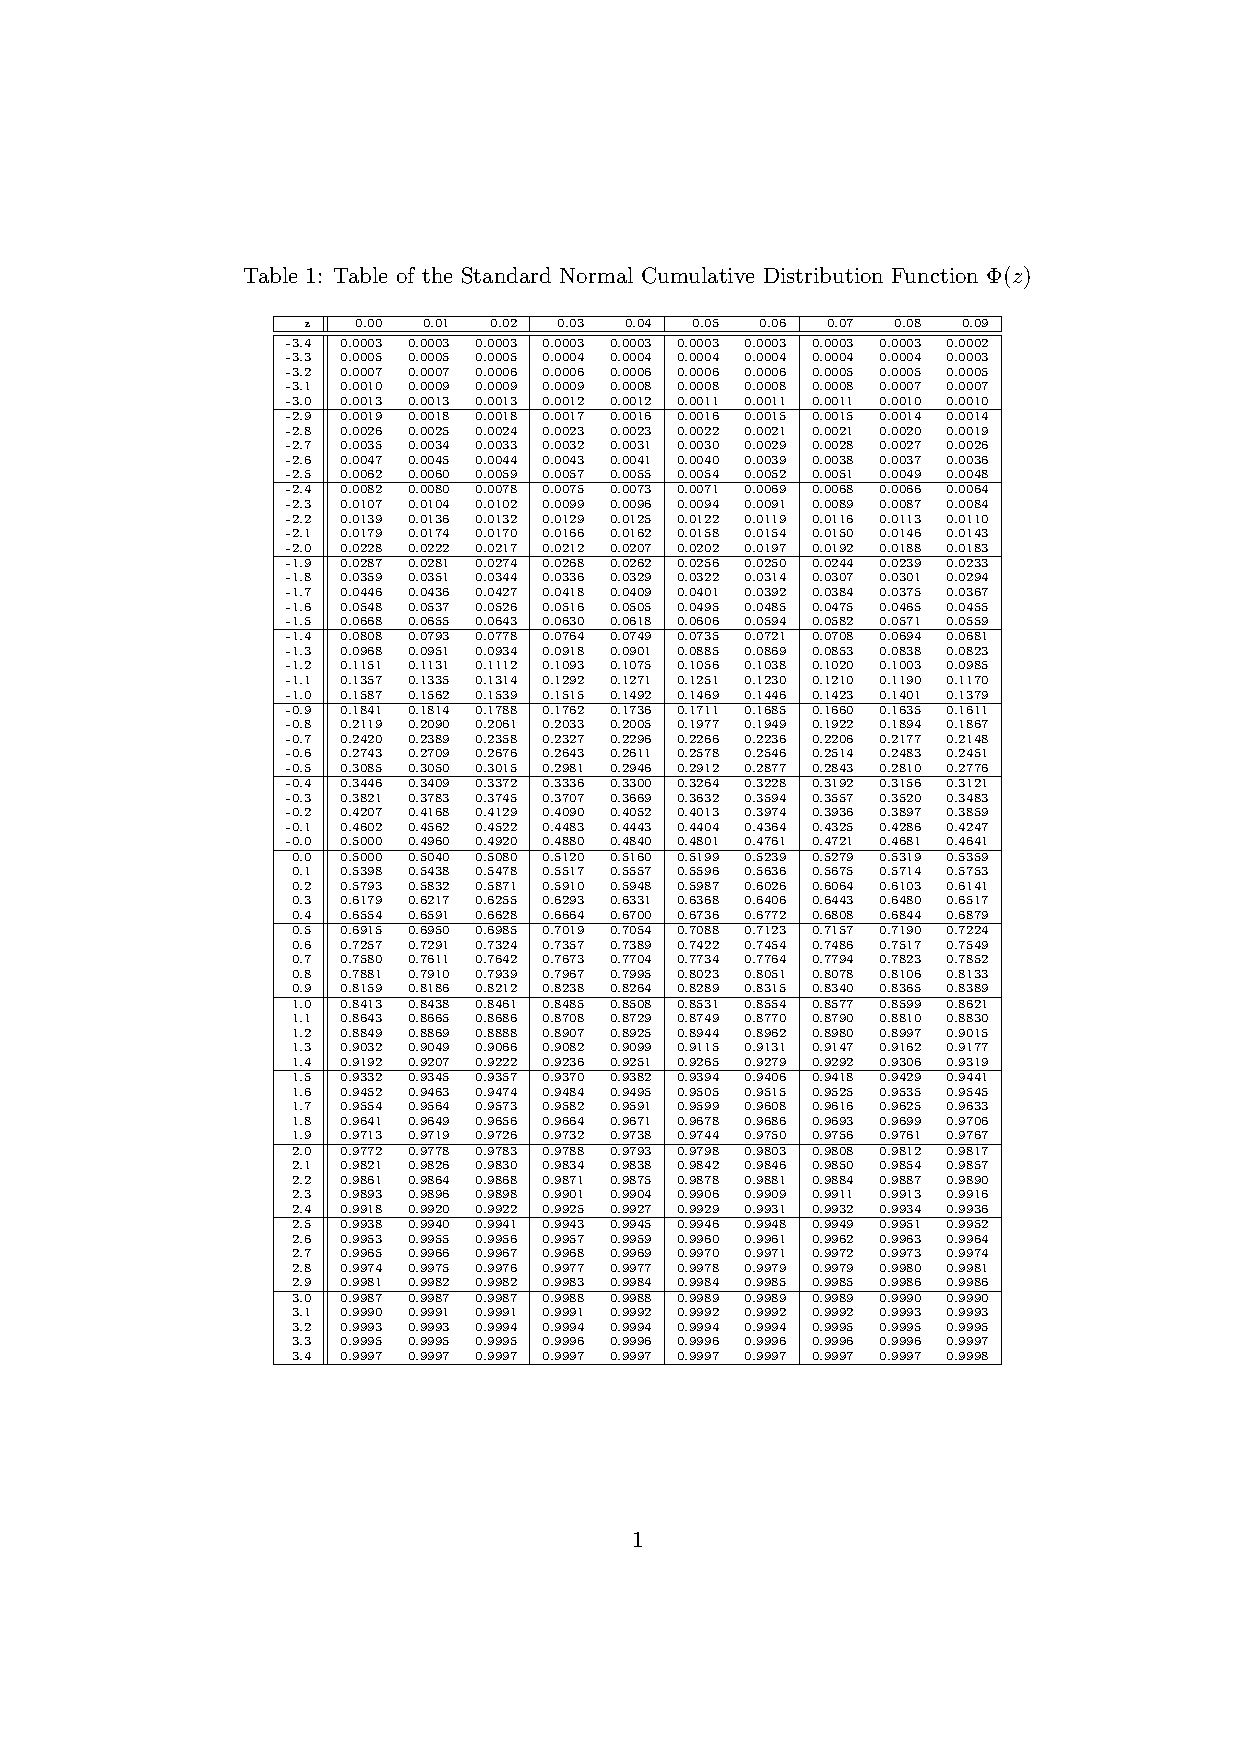
\includegraphics[width=\textwidth, center]{normal_cdf.pdf}
\iffalse
\section{Delta Function, Mixed (Being Discrete and Continuous at the same time) Random Variables
% (\textcolor{red}{Only for Engineering Students})
}
\begin{definition}[Unit Impulse (Delta) Function]
    Let
    \[d_{\epsilon}(x)={
        \begin{cases}
            1/\epsilon & -\epsilon/2\leq x\leq \epsilon/2 \\
            0 & otherwise.
        \end{cases}
    }\]
    The \textbf{unit impulse function} is
    \[\delta(x)=\lim_{\epsilon\rightarrow 0}d_{\epsilon}(x).\]
    Since
    \[\int_{-\infty}^{\infty}\delta(x)\diff x = 1.\]
    The $\delta(x)$ is indeed a PDF given it is also non-negative.
\end{definition}

\begin{theorem}
    For any continuous function $g(x)$,
    \[\int_{-\infty}^{\infty}g(x)\delta(x-x_0)\diff x = g(x_0).\]
\end{theorem}

\begin{definition}[Unit Step Function]
    The \textbf{unit step function} is
    \[u(x)={
        \begin{cases}
            0 & x<0, \\
            1 & x\geq 0.
        \end{cases}
    }\]
\end{definition}

\begin{theorem}[CDF of $\delta(x)$ and connection to the unit step function]\label{delta}
    \[\int_{-\infty}^{x}\delta(v)\diff v = u(x).\]
    And thus
    \[\delta(x)=\frac{\diff u(x)}{\diff x}.\]
\end{theorem}

\begin{corollary}
    The~\cref{delta} allows us to define a generalized \emph{PDF} that applies to discrete random variables as well as to continuous random variables. Consider the \emph{CDF} of a discrete random variable, $X$. It is constant (let's say $0$ for now) everywhere except at point $x_i\in S_X$, where it has jumps of height $P_X(x_i)$. Using the unit step function, the \emph{CDF} of $X$ is
    \[F_X(x)=\sum_{x_i\in S_X} P_X(x_i)u(x-x_i).\]
    And the \emph{PDF} can be defined with $\delta(x)$ as
    \[f_X(x)=\sum_{x_i\in S_X}P_X(x_i)\delta(x-x_i).\]
    Then the \emph{Expectation} will be
    \begin{align*}
        \E{X} &= \int_{-\infty}^{\infty}x\sum_{x_i\in S_X}P_X(x_i)\delta(x-x_i)\diff x \\
        \E{X} &= \sum_{x_i\in S_X}\int_{-\infty}^{\infty}xP_X(x_i)\delta(x-x_i)\diff x = \sum_{x_i\in S_X}x_i P_X(x_i)
    \end{align*}
\end{corollary}

\begin{theorem}
    For a random variable $X$ (not specified whether it is discrete or continuous), we have
    \begin{align*}
        q
        &= \P{X=x_0}  \tag{General expression} \\
        &= P_X(x_0)  \tag{PMF} \\
        &= F_X(x_0^+) - F_X(x_0^-)  \tag{CDF} \\
        &= f_X(x_0)  \tag{(PDF)} \\
        &= q\delta(0).  \tag{Delta function}
    \end{align*}
\end{theorem}

\begin{theorem}
    $X$ is a \textbf{mixed} random variable if and only if $f_X(x)$ contains both impulses and nonzero, finite values.
\end{theorem}
\fi